\subsubsection{Dátový formát}
Jedným z hlavných problémov pri spracovaní sekvenovaných dát je rozdiel medzi formátom, v ktorom sú dáta publikované, a formátom vhodným na ďalšiu analýzu.
Vstupné dáta boli dostupné najmä vo formáte \texttt{pod5}, ktorý obsahuje surový elektrický signál z nanopórového sekvenovania.
Tento surový signál je potrebné preložiť do DNA sekvencií, ktoré sú následne použiteľné na klastrovanie a viacnásobné zarovnanie.

\begin{figure}[htbp]
\centering
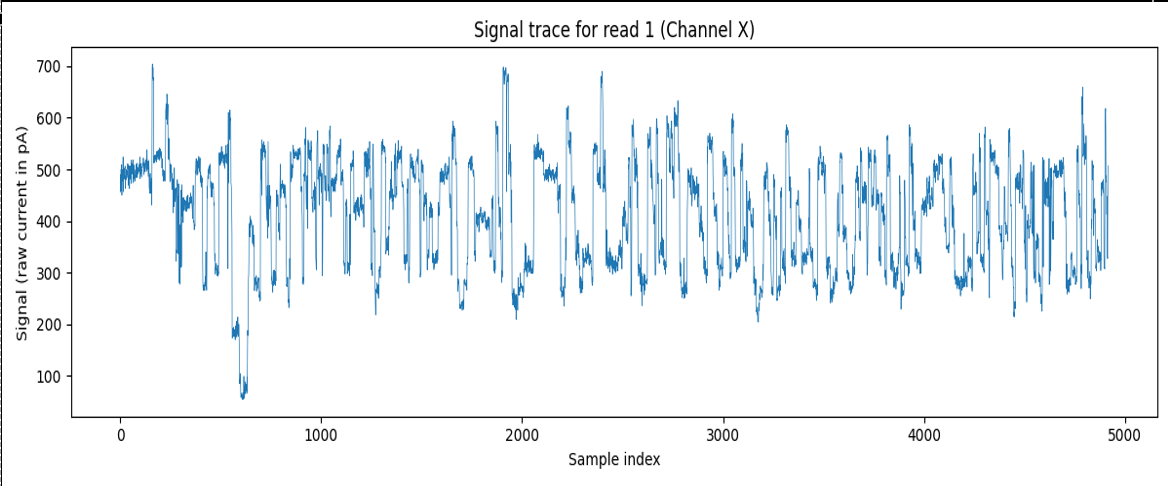
\includegraphics[width=0.95\textwidth]{chapters/Figures/Pod5Signal1}
\caption{Príklad surového signálu z nanopórového senzora – signal trace pre jeden kanál. Graf znázorňuje elektrický prúd (v pA) meraný v čase počas prechodu DNA molekuly nanopórom.}
\label{fig:pod5_signal1}
\end{figure}

Po preklade signálu nástrojom Dorado vzniká výstup vo formáte \texttt{BAM}, ktorý síce obsahuje prečítané sekvencie, avšak pre ďalšie kroky bolo potrebné údaje transformovať do jednoduchšieho textového tvaru.

Dáta spracované klastrovaním algoritmom Clover poskytovali výstup v špecifickom formáte, ktorý bolo potrebné ďalej spracovať, aby bolo možné získať samotné klastre a následne ich zarovnať a získať konsenzus.

Spracovávané dáta boli rozsiahle, ich sťahovanie trvalo dlhý čas a spracovanie nástrojom Dorado basecallerom trvalo približne pol dňa v najrýchlejšom režime. Bolo tiež potrebné stiahnuť predinštalovaný nástroj Dorado, ktorý zaberal značné množstvo miesta v pamäti.
